\noindent This supplementary material is organized as follows: 
\begin{itemize}
    \item Section \ref{architecture} demonstrates the detailed architecture of our baseline models in three tasks and how to insert our adapters into them.
    \item Section \ref{hyperparameters} details the training hyperparameters adopted in our experiments. 
    \item Section \ref{category} details per-class experimental results. 
\end{itemize}


\section{Detailed Architecture}\label{architecture}
We illustrate the architectures of both image and point cloud backbones and show how to insert the memory-based adapters into them in Figure \ref{arch}.
For online 3D semantic segmentation, we use U-Net~\cite{ronneberger2015u} as the image backbone and Minkowski-UNet~\cite{choy20194d} as the point cloud backbone, which is shown in Figure \ref{arch} (D) and (C) respectively.
For online 3D object detection, we adopt ResNet~\cite{he2016deep} with FPN~\cite{lin2017fpn} as the image backbone and FCAF3D~\cite{rukhovich2022fcaf3d} as the point cloud backbone, which is shown in Figure \ref{arch} (E) and (B) respectively.
For online 3D instance segmentation, we use the same image backbone as the object detection task and adopt TD3D~\cite{kolodiazhnyi2023top} as the point cloud backbone, which is shown in Figure \ref{arch} (E) and (A) respectively.
Note that for TD3D, the backbone maintains a high-resolution scene representation for ROI-wise instance prediction. We consrtuct a point cloud memory to cache this scene representation, which ensures the point clouds within each ROI are the most complete up to current time. This design helps us acquire complete instance mask by simply performing 3D NMS, which avoids complicated mask fusion strategy~\cite{liu2022ins} to merge instance masks of different frames.


\begin{figure}[t]
    \centering
    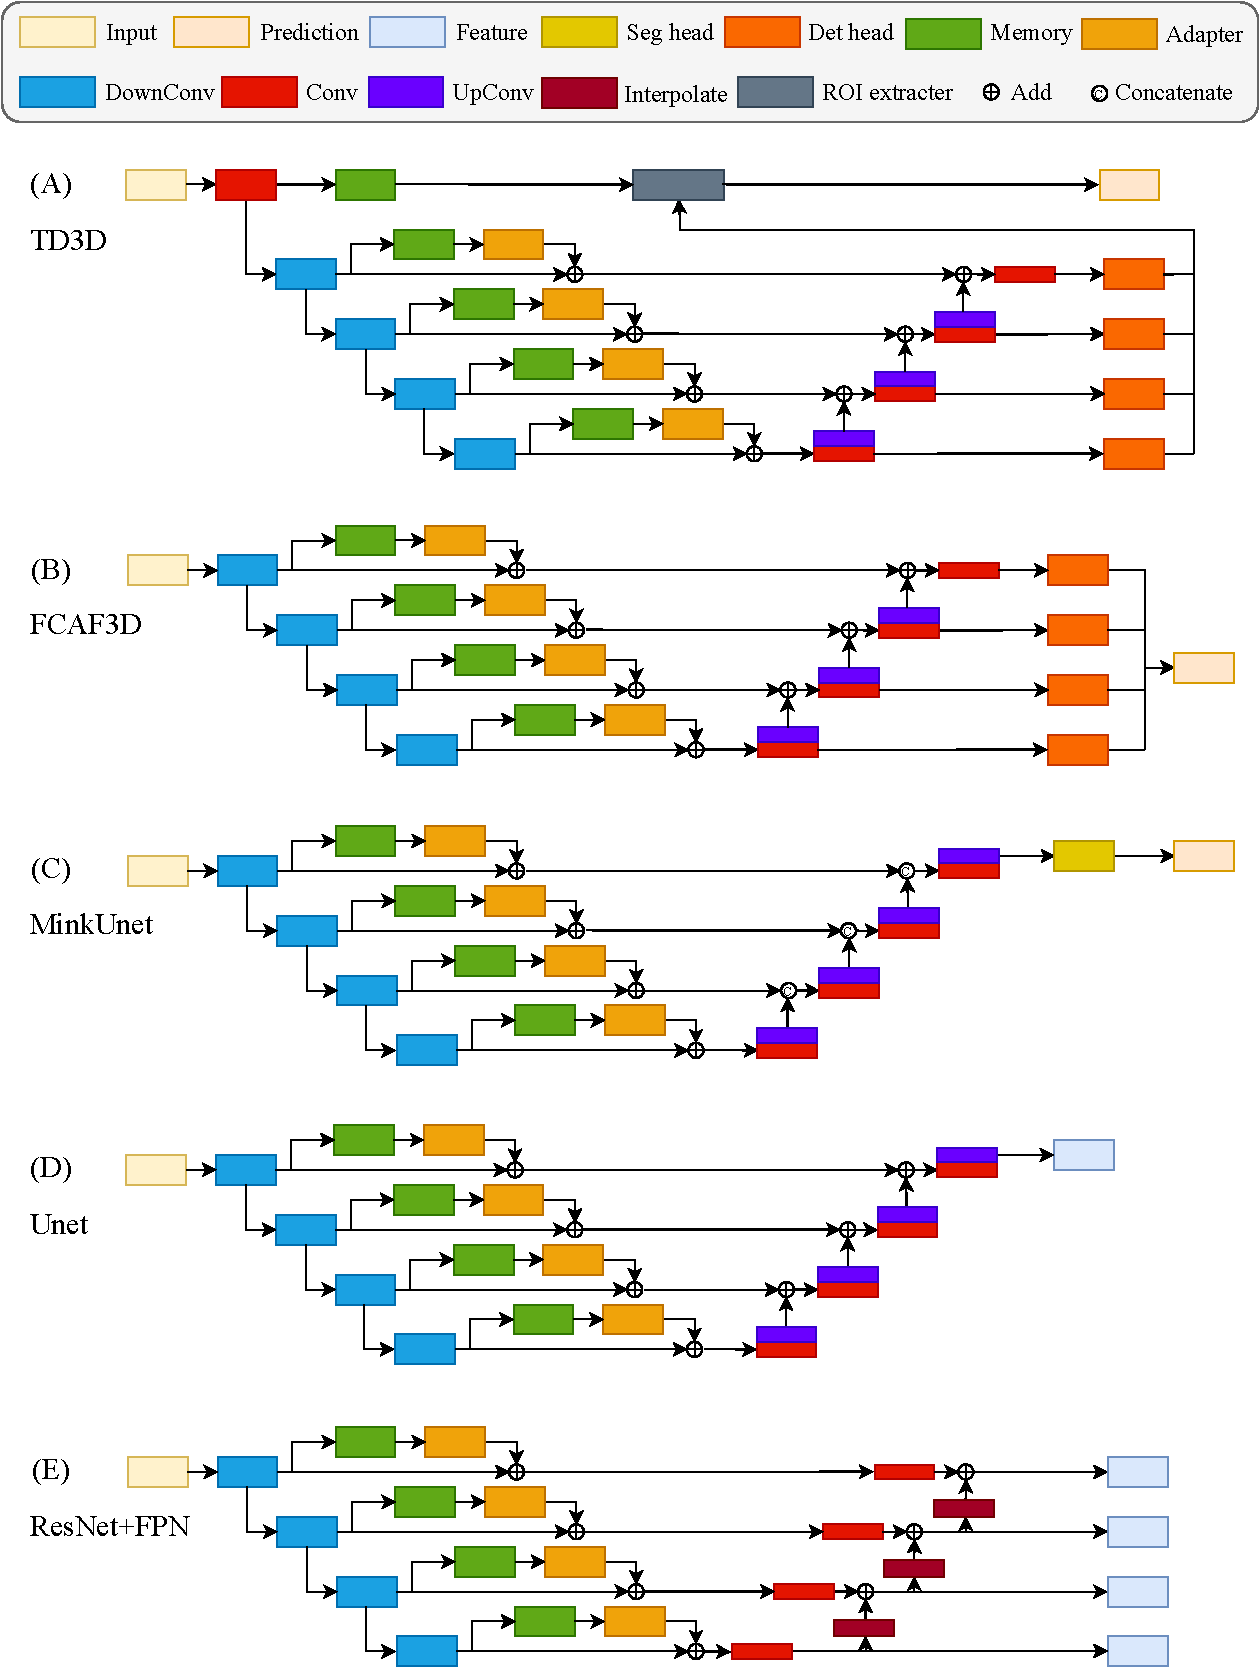
\includegraphics[width=1.0\linewidth]{figures/supp.pdf}
    \caption{Details about the architectures of image and point cloud backbones and how to insert the adapters into them.}
    \label{arch}
\end{figure}


\section{Training Hyperparameters}\label{hyperparameters}
We train the online perception models in two stage. Firstly we train single-view perception model $\mathcal{M}_{SV}$ on ScanNet-25k~\cite{dai2017scannet}. 
% with a fixed image backbone $\mathcal{M}_{I}$ pretrained by Pri3D~\cite{hou2021pri3d}. 
Secondly we insert the memory-based adapters into $\mathcal{M}_{SV}$ and finetune the network on ScanNet RGB-D videos.

For online semantic segmentation, we set max epoch as 250, weight decay as 0.01, initial learning rate as 0.0008 and adopt AdamW optimizer with OneCycleLR scheduler for the first stage. Then we set max epoch as 36, weight decay as 0.01, initial learning rate as 0.008 and adopt AdamW optimizer with a stepwise scheduler which steps at 24 and 32 epoch for the second stage.

For online object detection, we set max epoch as 12, weight decay as 0.0001, initial learning rate as 0.001 and adopt AdamW optimizer with a stepwise scheduler which steps at 8 and 11 epoch for the first stage. Then we adopt the same hyperparameters for finetuning in the second stage.

For online instance segmentation, we set max epoch as 33, weight decay as 0.0001, initial learning rate as 0.001 and adopt AdamW optimizer with a stepwise scheduler which steps at 28 and 32 epoch for the first stage. Then we adopt the same hyperparameters for finetuning.


\section{Class-specific Results}\label{category}
We provide class-specific experimental results of out method on three 3D scene perception tasks. Table \ref{supp:tab1} and \ref{supp:tab2} show the 3D semantic segmentation results on ScanNet and SceneNN dataset with per-class IoU. 
Table \ref{supp:tab3} and \ref{supp:tab4} show the 3D object detection results on ScanNet dataset with per-class AP$_{25}$ and AP$_{50}$.
Table \ref{supp:tab5} and \ref{supp:tab6} show the 3D object detection results on ScanNet dataset with per-class AP$_{25}$ and AP$_{50}$.

\newpage

\begin{table*}[tp]
	\centering
	\caption{Per-class 3D semantic segmentation results (IoU) of our method on the ScanNet validation set.}
        \vspace{-6pt}
	\scalebox{0.8}{\setlength{\tabcolsep}{0.3mm}{
	\begin{tabular}{@{}cccccccccccccccccccccc@{}}
		\toprule
		     & wall   & floor & cabinet & bed   & chair & sofa  & table & door  & window & bookshelf & picture &         counter & desk  &  curtain & fridge & curtain & toilet & sink  & bathtub & others & mean \\ 
            \midrule
            Ours   & 85.7  & 97.1 & 63.1  & 80.7 & 89.0 & 76.1 & 73.7   & 66.1  & 63.6    & 77.1     & 41.8     & 65.5   & 61.2 & 58.9   & 61.0       & 72.7    & 95.2  & 77.9 & 94.2   & 53.6 &72.7    \\     
            \bottomrule

    \end{tabular}}}
	\label{supp:tab1}\vspace{-8pt}
\end{table*} 

\begin{table*}[tp]
	\centering
	\caption{Per-class 3D semantic segmentation results (IoU) of our method on the SceneNN validation set.}
        \vspace{-6pt}
	\scalebox{0.8}{\setlength{\tabcolsep}{0.3mm}{
	\begin{tabular}{@{}cccccccccccccccccc@{}}

		\toprule
		     & wall   & floor & cabinet & bed   & chair & sofa  & table & door  & window & bookshelf & picture &         counter & desk  &  curtain & fridge  & sink  & mean \\ 
            \midrule
            Ours   & 75.3  & 82.6 & 59.8  & 82.8 & 62.0 & 57.8 & 18.4   & 52.4  & 20.5    & 55.9     & 29.4     & 52.6   & 44.9 & 50.2   & 80.3       & 81.8    & 56.7   \\     
            \bottomrule
    \end{tabular}}}
	\label{supp:tab2}\vspace{-8pt}
\end{table*} 


\begin{table*}[tp]
	\centering
	\caption{Per-class 3D object detection results (AP$_{25}$) of our method on the ScanNet validation set.}
        \vspace{-6pt}
	\scalebox{0.8}{\setlength{\tabcolsep}{0.3mm}{
	\begin{tabular}{@{}ccccccccccccccccccccc@{}}
		\toprule
		  & cabinet & bed   & chair & sofa  & table & door  & window & bookshelf & picture & counter & desk  &  curtain & fridge & curtain & toilet & sink  & bathtub & others&mean \\ \midrule
        Ours           & 55.2  & 85.4 & 88.7  & 87.2 & 63.3 & 62.5 & 47.3   & 66.2  & 36.0    & 65.2     & 80.1     & 65.0   & 58.1 & 76.3   & 99.7       & 76.7    & 93.3  & 62.0 &70.5   \\     \bottomrule
    \end{tabular}}}
	\label{supp:tab3}\vspace{-8pt}
\end{table*} 


\begin{table*}[tp]
	\centering
	\caption{Per-class 3D object detection results (AP$_{50}$) of our method on the ScanNet validation set.}
        \vspace{-6pt}
	\scalebox{0.8}{\setlength{\tabcolsep}{0.3mm}{
	\begin{tabular}{@{}ccccccccccccccccccccc@{}}
		\toprule
		  & cabinet & bed   & chair & sofa  & table & door  & window & bookshelf & picture & counter & desk  &  curtain & fridge & curtain & toilet & sink  & bathtub & others&mean \\ \midrule
        Ours           & 36.7  & 75.6 & 73.9  & 77.9 & 57.0 & 33.8 & 19.8   & 43.7  & 19.4    & 26.3     & 62.8     & 32.4   & 41.1 & 24.6   & 89.2       & 46.7    & 84.8  & 52.2 &49.9   \\     \bottomrule
    \end{tabular}}}
	\label{supp:tab4}\vspace{-8pt}
\end{table*} 


\begin{table*}[tp]
	\centering
	\caption{Per-class 3D instance segmentation results (AP$_{25}$) of our method on the ScanNet validation set.}
        \vspace{-6pt}
	\scalebox{0.8}{\setlength{\tabcolsep}{0.3mm}{
	\begin{tabular}{@{}ccccccccccccccccccccc@{}}
		\toprule
		  & cabinet & bed   & chair & sofa  & table & door  & window & bookshelf & picture & counter & desk  &  curtain & fridge & curtain & toilet & sink  & bathtub & others&mean \\ \midrule
        Ours           & 60.3  & 86.8 & 91.5  & 80.3 & 72.8 & 56.0 & 55.3   & 67.5  & 45.1    & 48.9     & 72.9     & 68.4   & 56.5 & 86.3   & 99.7       & 81.3    & 87.8  & 65.3 &71.3   \\     \bottomrule
    \end{tabular}}}
	\label{supp:tab5}\vspace{-8pt}
\end{table*} 


\begin{table*}[tp]
	\centering
	\caption{Per-class 3D instance segmentation results (AP$_{50}$) of our method on the ScanNet validation set.}
        \vspace{-6pt}
	\scalebox{0.8}{\setlength{\tabcolsep}{0.3mm}{
	\begin{tabular}{@{}ccccccccccccccccccccc@{}}
		\toprule
		  & cabinet & bed   & chair & sofa  & table & door  & window & bookshelf & picture & counter & desk  &  curtain & fridge & curtain & toilet & sink  & bathtub & others&mean \\ \midrule
        Ours           & 50.9  & 79.1 & 82.5  & 71.3 & 63.6 & 44.0 & 36.0   & 45.5  & 38.5    & 30.3     & 57.3     & 49.8   & 52.9 & 78.9   & 99.7       & 66.6    & 84.9  & 56.9 & 60.5   \\     \bottomrule
    \end{tabular}}}
	\label{supp:tab6}\vspace{-8pt}
\end{table*} 
